%% Supporting Information
\documentclass[journal=jcisd8,manuscript=suppinfo]{achemso}

\usepackage[T1]{fontenc}
\usepackage{amsmath,amssymb}
\usepackage{booktabs}
\usepackage{graphicx}

\SectionNumbersOn

\author{Talha Kırca}
\email{talhakirca@kmu.edu.tr}
\affiliation{Department of Data Science and Analytics, Karamanoğlu Mehmetbey University, 70200 Karaman, Türkiye}
\author{Hasan Yıldırım}
\affiliation{Department of Data Science and Analytics, Karamanoğlu Mehmetbey University, 70200 Karaman, Türkiye}
\author{Merve Görgülü}
\affiliation{Department of Data Science and Analytics, Karamanoğlu Mehmetbey University, 70200 Karaman, Türkiye}

\title[Supporting Information]
{Supporting Information: Graph Network Attributions Track Atom Degree Before Training}

\begin{document}

\maketitle

\section{The alert library}

Table~\ref{tab:si_smarts} lists the eighteen SMARTS patterns, how many of the 237 evaluation
molecules each matches, and the share of all alert atoms it contributes. The two columns tell
different stories. The pattern for fused aromatic systems matches fewer than half the
molecules but supplies more than three fifths of the atoms the agreement measure is scored
against, because it matches whole ring systems while the heteroatom patterns match small
groups. Any single agreement figure computed over the full library is therefore weighted
heavily toward that one pattern.

\begin{table}[htbp]
\centering
\caption{The eighteen structural alerts, with the number of the 237 evaluation molecules each matches and its share of all alert atoms. Shares sum to more than 100\% because patterns overlap.}
\label{tab:si_smarts}
\small
\setlength{\tabcolsep}{4pt}
\begin{tabular}{llcc}
\toprule
Alert & SMARTS & Molecules & Share of alert atoms \\
\midrule
polycyclic aromatic & \texttt{\detokenize{c1ccc2ccccc2c1}} & 97 & 61.8 \\
aromatic amine & \texttt{\detokenize{[a][NX3;H2,H1;!$(N[!#6]);!$(N=*)]}} & 50 & 6.2 \\
epoxide & \texttt{\detokenize{C1OC1}} & 43 & 7.0 \\
aromatic nitro & \texttt{\detokenize{[a][N+](=O)[O-]}} & 32 & 7.1 \\
michael acceptor & \texttt{\detokenize{[CX3]=[CX3][CX3]=[OX1]}} & 30 & 7.5 \\
aziridine & \texttt{\detokenize{C1NC1}} & 15 & 2.7 \\
aliphatic halide & \texttt{\detokenize{[CX4][F,Cl,Br,I]}} & 10 & 2.1 \\
azo aromatic & \texttt{\detokenize{[a][NX2]=[NX2][a]}} & 8 & 3.3 \\
nitrogen mustard & \texttt{\detokenize{[NX3]([CX4][CX4][F,Cl,Br,I])[CX4][CX4][F,Cl,Br,I]}} & 7 & 2.2 \\
nitrosamine & \texttt{\detokenize{[NX3][NX2]=[OX1]}} & 5 & 1.0 \\
alkyl sulfonate & \texttt{\detokenize{[CX4][OX2][SX4](=[OX1])(=[OX1])}} & 3 & 0.7 \\
hetero hetero bond & \texttt{\detokenize{[N,O;H1,H2][N,O;H1,H2]}} & 3 & 0.3 \\
azide & \texttt{\detokenize{[NX2]=[NX2+]=[NX1-]}} & 3 & 0.4 \\
aromatic hydrazine & \texttt{\detokenize{[a][NX3;H1][NX3;H2]}} & 1 & 0.1 \\
alkyl nitrite & \texttt{\detokenize{[CX4][OX2][NX2]=[OX1]}} & 0 & 0.0 \\
aromatic nitroso & \texttt{\detokenize{[a][NX2]=[OX1]}} & 0 & 0.0 \\
aromatic hydroxylamine & \texttt{\detokenize{[a][NX3;H1][OX2;H1]}} & 0 & 0.0 \\
aromatic azoxy & \texttt{\detokenize{[a][NX2]=[NX3+]([O-])[a]}} & 0 & 0.0 \\
\bottomrule
\end{tabular}
\begin{flushleft}\footnotesize The pattern matching fused aromatic systems is composed entirely of carbon; the remaining seventeen are centred on heteroatoms, of which thirteen match anything here. The two groups reward opposite rankings, so a single agreement figure averages two regimes.\end{flushleft}
\end{table}


\section{Data and search budget}

Table~\ref{tab:si_data} records the curation of the benchmark and the composition of the
designated partition.

\begin{table}[htbp]
\centering
\caption{Curation of the benchmark and composition of the designated partition used for the attribution analyses. Scaffold partitioning does not preserve the mutagenic fraction.}
\label{tab:si_data}
\small
\setlength{\tabcolsep}{4pt}
\begin{tabular}{lr}
\toprule
Quantity & Value \\
\midrule
Compounds retrieved & 7,255 \\
Unparseable structures removed & 0 \\
Contradictory duplicates removed & 0 \\
Redundant duplicates collapsed & 0 \\
Compounds analysed & 7,255 \\
Mutagenic fraction & 0.545 \\
Designated partition, train & 5,804 (55.6\% mutagenic) \\
Designated partition, valid & 725 (53.7\% mutagenic) \\
Designated partition, test & 726 (46.3\% mutagenic) \\
\bottomrule
\end{tabular}
\end{table}

Table~\ref{tab:si_hpo} gives the search budget and the selected configuration for every
model.

\begin{table}[htbp]
\centering
\caption{Hyperparameter search. Every model received the same number of trials over its own space, and the search and the final fits used one training protocol.}
\label{tab:si_hpo}
\small
\setlength{\tabcolsep}{4pt}
\begin{tabular}{lccc}
\toprule
Model & Trials & Validation ROC-AUC & Search time (min) \\
\midrule
XGBoost (ECFP4) & 100 & 0.839 & 2.185 \\
Random forest (ECFP4) & 100 & 0.833 & 15.259 \\
GCN & 100 & 0.849 & 63.140 \\
GIN & 100 & 0.852 & 69.288 \\
GAT & 100 & 0.847 & 104.779 \\
XGBoost (RDKit-2D) & 100 & -- & -- \\
Logistic regression (ECFP4) & 100 & -- & -- \\
GIN and GAT, no bond features & 100 & -- & -- \\
\bottomrule
\end{tabular}
\begin{flushleft}\footnotesize Recorded search time is 17.4 minutes for the two classical models timed and 237.2 for the three graph models, a ratio of 13.6 to 1. Timings for the descriptor model, the logistic regression and the ablated graph variants were not recorded, so the ratio is a lower bound on the classical side and should be read as an order of magnitude. Selected configurations are released as JSON.\end{flushleft}
\end{table}


Search spaces were the same for every model of a family. The gradient-boosted models were
searched over tree depth, learning rate, subsample and column-sample fractions, minimum child
weight and the two regularisation terms; the random forest over the number of trees, depth,
and the split criteria; the graph models over hidden width, number of layers, dropout,
learning rate, weight decay, batch size and the use of residual connections. Selected
configurations are released as JSON with the pipeline.

\section{Model comparison}

Table~\ref{tab:si_pairwise} gives all fifteen pairwise differences among the six main models
on the out-of-fold predictions, with Holm-corrected $p$-values.

\begin{table}[htbp]
\centering
\caption{Pairwise differences between the six main models on the out-of-fold predictions.}
\label{tab:si_pairwise}
\small
\setlength{\tabcolsep}{4pt}
\begin{tabular}{llccc}
\toprule
Model A & Model B & $\Delta$ & 95\% CI & $p$ (Holm) \\
\midrule
XGBoost (ECFP4) & Random forest (ECFP4) & +0.0116 & +0.0067 to +0.0164 & $<0.001$ \\
XGBoost (ECFP4) & XGBoost (RDKit-2D) & -0.0129 & -0.0195 to -0.0064 & 0.001 \\
XGBoost (ECFP4) & GCN & -0.0105 & -0.0179 to -0.0031 & 0.021 \\
XGBoost (ECFP4) & GIN & -0.0130 & -0.0198 to -0.0062 & $<0.001$ \\
XGBoost (ECFP4) & GAT & -0.0216 & -0.0289 to -0.0144 & $<0.001$ \\
Random forest (ECFP4) & XGBoost (RDKit-2D) & -0.0244 & -0.0311 to -0.0180 & $<0.001$ \\
Random forest (ECFP4) & GCN & -0.0221 & -0.0307 to -0.0136 & $<0.001$ \\
Random forest (ECFP4) & GIN & -0.0245 & -0.0322 to -0.0168 & $<0.001$ \\
Random forest (ECFP4) & GAT & -0.0332 & -0.0416 to -0.0249 & $<0.001$ \\
XGBoost (RDKit-2D) & GCN & +0.0023 & -0.0048 to +0.0096 & 1.000 \\
XGBoost (RDKit-2D) & GIN & -0.0001 & -0.0068 to +0.0067 & 1.000 \\
XGBoost (RDKit-2D) & GAT & -0.0088 & -0.0158 to -0.0016 & 0.056 \\
GCN & GIN & -0.0024 & -0.0082 to +0.0033 & 1.000 \\
GCN & GAT & -0.0111 & -0.0162 to -0.0062 & $<0.001$ \\
GIN & GAT & -0.0087 & -0.0142 to -0.0030 & 0.008 \\
\bottomrule
\end{tabular}
\end{table}


\section{Attribution}

Table~\ref{tab:si_explainers} reports the four attribution methods on the designated
partition using one representative model, which is how such comparisons are usually made. This model is not one of the twenty
fitted later for the architecture comparison: it is the first of the three seeds used
throughout Parts 2 to 5, fixed before any attribution was computed. Its agreement of $1.226$
falls below the mean of the twenty, $1.265$, so figures computed on it are not
interchangeable with the distribution the main text reports, and the two sets are named
separately wherever both appear. The
main text reports the same measurements across twenty models, and the difference between the
two is the point of the corresponding section of the manuscript.

\begin{table}[htbp]
\centering
\caption{Attribution methods on the designated partition, using one representative trained model. Characterisation is the fidelity score under node removal; Jaccard is the agreement of the top 30\% over five repeats.}
\label{tab:si_explainers}
\footnotesize
\setlength{\tabcolsep}{4pt}
\begin{tabular}{lccccc}
\toprule
Method & Lift & AUROC & $p$ (Holm) & Charact. & Jaccard \\
\midrule
TreeSHAP & 1.542 [1.462, 1.633] & 0.798 & $<0.001$ & -- & -- \\
Integrated Gradients & 1.226 [1.171, 1.284] & 0.615 & $<0.001$ & 0.582 & 0.987 \\
Gradient $\times$ Input & 1.216 [1.151, 1.284] & 0.605 & $<0.001$ & 0.582 & -- \\
Saliency & 1.178 [1.105, 1.259] & 0.613 & $<0.001$ & 0.630 & -- \\
GNNExplainer & 0.898 [0.845, 0.952] & 0.476 & 0.032 & 0.233 & 0.629 \\
\bottomrule
\end{tabular}
\end{table}


Figure~\ref{fig:si_protocol} contrasts the design a single untrained control supports with the
one adopted here.

\begin{figure}[htbp]
\centering
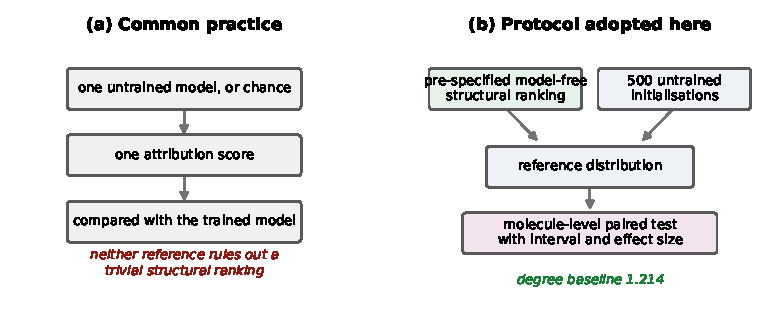
\includegraphics[width=\textwidth]{figures/figS3_protocol.pdf}
\caption{The common design for a negative control, and the design used in this work.}
\label{fig:si_protocol}
\end{figure}

Agreement is reported in the main text at a retained fraction of 30\% of atoms.
Figure~\ref{fig:si_topk} shows the arms across fractions. The trained model lies within the
central 95\% of the untrained draws at four of the five fractions and marginally above it at
the smallest, where it reaches $1.362$ against an upper bound of $1.354$. Its margin over the
degree ranking is not constant across fractions, and the main text reports that dependence
with intervals.

\begin{figure}[htbp]
\centering
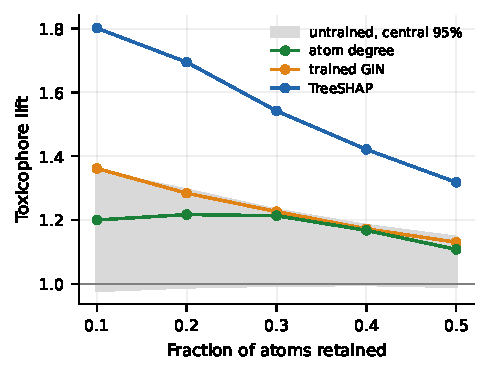
\includegraphics[width=0.62\textwidth]{figures/figS6_topk.pdf}
\caption{Agreement across retained fractions. The shaded band is the central 95\% of 500
untrained initialisations.}
\label{fig:si_topk}
\end{figure}

Figure~\ref{fig:si_epoch} follows agreement and validation performance together over the
course of training, averaged across five runs.

\begin{figure}[htbp]
\centering
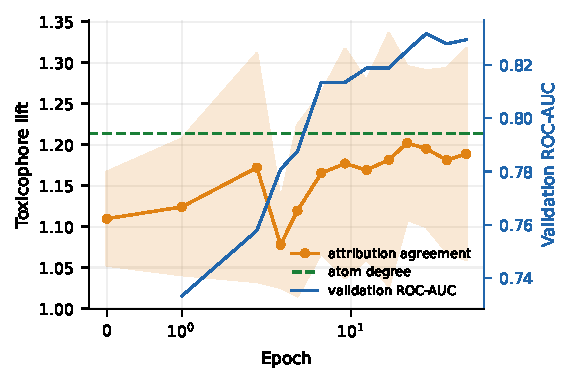
\includegraphics[width=0.62\textwidth]{figures/figS7_epoch.pdf}
\caption{Toxicophore agreement and validation ROC-AUC over training, averaged over five runs.
The shaded band is one standard deviation across runs. Agreement plateaus while predictive performance
continues to improve. The plateau lies below the value reached by the fully trained models of
the main text, which are selected by early stopping and may run far beyond the epochs
sampled here.}
\label{fig:si_epoch}
\end{figure}

\section{Negative controls}

Table~\ref{tab:si_permutation} reports the permutation control for both model families.

\begin{table}[htbp]
\centering
\caption{Permutation control. Labels were permuted and each model fitted with regularisation and early stopping switched off, escalating the budget until the randomised labels were absorbed.}
\label{tab:si_permutation}
\footnotesize
\setlength{\tabcolsep}{4pt}
\begin{tabular}{lccccc}
\toprule
Family & Repeats & Absorbed & Training ROC-AUC & Test ROC-AUC & Lift \\
\midrule
Graph (GIN) & 14 & 14 & 0.874 & 0.492 & 1.036 $\pm$ 0.074 \\
Tree (XGBoost) & 16 & 16 & 0.973 & 0.494 & 0.995 $\pm$ 0.054 \\
\bottomrule
\end{tabular}
\begin{flushleft}\footnotesize Training ROC-AUC is measured on the permuted labels and test ROC-AUC against the true labels. A model that has not absorbed the randomised labels tests nothing beyond an untrained one.\end{flushleft}
\end{table}


A model fitted to permuted labels is informative as a control only if it has fitted them.
Regularisation and early stopping were therefore switched off and the budget escalated until
the training ROC-AUC on the permuted target rose above 0.60 with a non-degenerate prediction
distribution. The two arms are not matched. The graph arm carries fourteen repeats and the tree arm
sixteen, and the two absorbed their randomised labels to different degrees, $0.874$ against
$0.973$ in training ROC-AUC. A comparison between the families on this control should
therefore be read as indicative rather than as a matched contrast.

Runs that collapse to a constant output produce a random atom ranking and a
lift of one by construction and test nothing. Under the escalation described above every
graph repeat eventually absorbed its labels, so none was excluded.

\section{Attribution rule and representation}

Table~\ref{tab:si_2x2} separates the attribution rule from the molecular representation.

\begin{table}[htbp]
\centering
\caption{The attribution rule and the molecular representation, separated. Applying Integrated Gradients to a network over the same fingerprints, through the same bit-to-atom map, fills the missing cell of the design.}
\label{tab:si_2x2}
\small
\setlength{\tabcolsep}{4pt}
\begin{tabular}{lllc}
\toprule
Representation & Rule & Convention & Lift \\
\midrule
Molecular graph & Integrated Gradients & Absolute & 1.226 \\
Molecular graph & Integrated Gradients & Signed & 1.068 \\
Molecular graph & Gradient $\times$ Input & Absolute & 1.216 \\
Molecular graph & Gradient $\times$ Input & Signed & 1.170 \\
Molecular graph & Saliency & Absolute & 1.178 \\
Molecular graph & Saliency & Signed & 1.092 \\
Fingerprint & TreeSHAP & Absolute & 1.442 \\
Fingerprint & TreeSHAP & Signed & 1.542 \\
Fingerprint & Integrated Gradients & Absolute & 1.169 \\
Fingerprint & Integrated Gradients & Signed & 1.417 \\
\bottomrule
\end{tabular}
\begin{flushleft}\footnotesize The fingerprint network reaches 0.767 test ROC-AUC. Neither axis dominates, and the aggregation convention interacts with the representation.\end{flushleft}
\end{table}


The two arms compared in the main text differ on two axes at once. Circular fingerprint bits
are substructure counters and the alerts are substructures, so the fingerprint arm is aligned
with the target by construction. Applying Integrated Gradients to a network over the same
fingerprints, and mapping the attributions to atoms through the same bit-to-atom
correspondence, fills the missing cell.

\section{Mask-based explanation}

Table~\ref{tab:si_gnnexplainer} reports mask-based explanation under three settings.

\begin{table}[htbp]
\centering
\caption{Mask-based explanation under three settings. Entropy is normalised to the number of atoms, so a value near one means the learned mask is close to uniform and the ranking it induces is arbitrary.}
\label{tab:si_gnnexplainer}
\small
\setlength{\tabcolsep}{4pt}
\begin{tabular}{lcccc}
\toprule
Setting & Models & Epochs & Lift & Mask entropy \\
\midrule
default & 5 & 100 & 0.970 $\pm$ 0.100 & 0.995 \\
longer & 5 & 300 & 1.060 $\pm$ 0.091 & 0.979 \\
weak\_reg & 5 & 100 & 0.911 $\pm$ 0.051 & 0.994 \\
\bottomrule
\end{tabular}
\end{table}


Mask entropy is normalised to the number of atoms in the molecule, so a value approaching one
means the learned mask is close to uniform. A near-uniform mask does not produce an
uninformative ranking so much as an arbitrary one, since the ordering it induces is then
governed by numerical noise rather than by the optimisation.

\section{The untrained distribution}

Table~\ref{tab:si_nullhp} gives the sensitivity of the untrained distribution to the size of
the network.

\begin{table}[htbp]
\centering
\caption{Sensitivity of the untrained distribution to the size of the network. No training is involved.}
\label{tab:si_nullhp}
\footnotesize
\setlength{\tabcolsep}{4pt}
\begin{tabular}{lccccc}
\toprule
Configuration & Hidden & Layers & Draws & Mean & SD \\
\midrule
selected & 64 & 4 & 200 & 1.113 & 0.061 \\
narrow shallow & 32 & 2 & 200 & 1.094 & 0.085 \\
wide deep & 256 & 5 & 200 & 1.132 & 0.055 \\
\bottomrule
\end{tabular}
\begin{flushleft}\footnotesize For comparison, the three architectures reported in the main text give standard deviations of 0.059 (GIN), 0.125 (GAT) and 0.141 (GCN).\end{flushleft}
\end{table}


The width of the untrained distribution differs markedly between architectures, from a
standard deviation of 0.059 for GIN to 0.141 for GCN. Two further configurations of the same
architecture, one narrower and shallower and one wider and deeper, do not reproduce that
range, so the difference is not explained by the size of the network. It remains unexplained.

\section{Calibration and conformal coverage}

Neural networks are systematically overconfident and temperature scaling largely repairs
it,\cite{guo2017calibration} uncertainty estimates in molecular property prediction have been
benchmarked,\cite{scalia2020uncertainty} and calibration in toxicological models has been
assessed with conformal prediction,\cite{bosc2021conformal,vovk2005} which is rarely reported
alongside accuracy on this endpoint. What follows is that reporting for the models compared
here.

The two families separate on calibration, and in opposite directions
(Figure~\ref{fig:si_cal}, Table~\ref{tab:calibration}). The random forest is
underconfident with a fitted temperature of $0.70$ and XGBoost on fingerprints at $0.77$,
while all three graph models sit above one, from $1.11$ for GCN to $1.46$ for GAT.
Temperature scaling repairs the graph models and slightly harms XGBoost, whose expected
calibration error rises from $0.059$ to $0.074$; the shift in class balance between the
validation and test sets that scaffold partitioning produces is the likely cause.

Under class-conditional conformal prediction at a nominal coverage of $0.90$ every model
undercovers, between $0.869$ and $0.879$. With 726 test compounds the differences between
models are not resolved, and which of them a given predictor flags depends on the predictor:
the class-conditional one flags XGBoost and GCN, the marginal one only GCN. We report the
general undercoverage and draw no conclusion about individual models.

Conformal validity requires exchangeability between the calibration and test sets, which
scaffold partitioning deliberately violates, and the designated partition also shifts the
class balance from 53.7\% to 46.3\% mutagenic. The undercoverage seen across all five
models is what that violation predicts, so the differences between models here should not be
read as differences in reliability.

One caveat limits how far this can be read. Every model was fitted with class weighting,
which shifts predicted probabilities before any temperature is applied, and the direction of
that shift differs between an averaged ensemble of trees and a network trained with a
weighted loss. The separation between the families is therefore not attributable to the
architecture alone.

\begin{figure}[htbp]
\centering
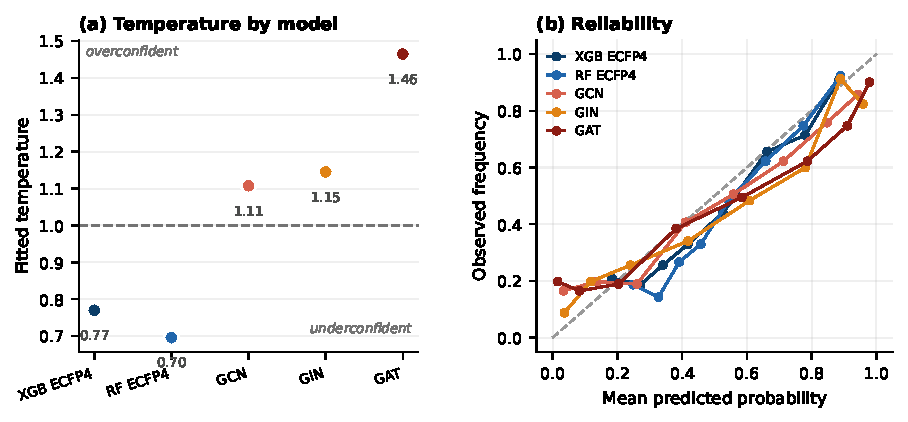
\includegraphics[width=0.85\textwidth]{figures/fig08_calibration.pdf}
\caption{(a) Fitted temperature on the designated partition; values above one indicate
overconfidence. (b) Reliability curves over eight equal-mass bins.}
\label{fig:si_cal}
\end{figure}

\begin{table}[htbp]
\centering
\caption{Calibration and class-conditional conformal coverage on the designated partition at a nominal level of 0.90.}
\label{tab:calibration}
\footnotesize
\setlength{\tabcolsep}{4pt}
\begin{tabular}{lccccc}
\toprule
Model & Temperature & ECE & ECE (scaled) & Coverage & Uncertain \\
\midrule
XGBoost (ECFP4) & 0.770 & 0.059 & 0.074 & 0.869 & 0.355 \\
Random forest (ECFP4) & 0.696 & 0.091 & 0.079 & 0.879 & 0.365 \\
GCN & 1.108 & 0.075 & 0.064 & 0.871 & 0.336 \\
GIN & 1.145 & 0.082 & 0.068 & 0.876 & 0.342 \\
GAT & 1.464 & 0.100 & 0.068 & 0.875 & 0.340 \\
\bottomrule
\end{tabular}
\begin{flushleft}\footnotesize Uncertain is the share of compounds for which no class can be asserted at the nominal level.\end{flushleft}
\end{table}


\section{Applicability domain}

The median nearest-neighbour Tanimoto similarity of a test compound to the training set is
$0.449$; at a threshold of $0.30$, 599 compounds fall inside the domain and 127 outside
(Figure~\ref{fig:si_adf}, Table~\ref{tab:ad}). Every model degrades outside, and at every
threshold from $0.15$ to $0.50$ the two classical models degrade more than the three graph
models. The pattern does not survive a test: a paired bootstrap over test compounds gives a
classical-minus-graph difference of $-0.048$ with a 95\% interval of $[-0.145, +0.043]$
($p = 0.35$). With 127 compounds outside the domain the comparison lacks the resolution to
support a claim in either direction.

\begin{figure}[htbp]
\centering
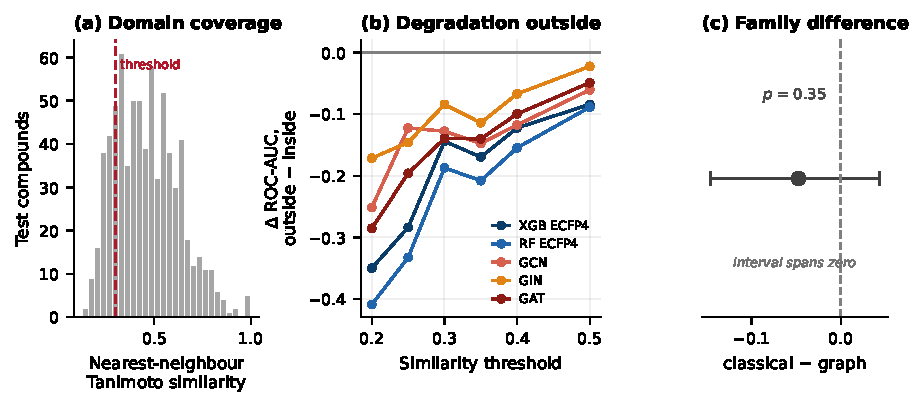
\includegraphics[width=0.85\textwidth]{figures/fig09_applicability.pdf}
\caption{(a) Distribution of nearest-neighbour similarity to the training set. (b)
Degradation outside the domain across thresholds. (c) The difference between the model
families, with its bootstrap interval.}
\label{fig:si_adf}
\end{figure}

\begin{table}[htbp]
\centering
\caption{Performance inside and outside the applicability domain, defined by a nearest-neighbour Tanimoto similarity of 0.30 to the training set.}
\label{tab:ad}
\small
\setlength{\tabcolsep}{4pt}
\begin{tabular}{lcccc}
\toprule
Model & Inside & Outside & $\Delta$ & Range \\
\midrule
XGBoost (ECFP4) & 0.797 & 0.653 & -0.144 & -0.35 to -0.08 \\
Random forest (ECFP4) & 0.816 & 0.629 & -0.187 & -0.41 to -0.09 \\
GCN & 0.801 & 0.673 & -0.128 & -0.25 to -0.06 \\
GIN & 0.819 & 0.734 & -0.084 & -0.17 to -0.02 \\
GAT & 0.812 & 0.673 & -0.140 & -0.29 to -0.05 \\
\bottomrule
\end{tabular}
\begin{flushleft}\footnotesize 599 compounds fall inside and 127 outside. A paired bootstrap gives a classical-minus-graph difference of -0.048 (95\% CI -0.145 to +0.043, $p$ = 0.35), so the families cannot be distinguished here.\end{flushleft}
\end{table}


\section{Decision rule}

Table~\ref{tab:si_rules} lists every comparison made against the degree ranking with the
correction family it belongs to, the test counts being read from the tables themselves rather
than stated here.

\begin{table}[htbp]
\centering
\caption{Every comparison made against the degree ranking, with its correction family and decision threshold.}
\label{tab:si_rules}
\small
\setlength{\tabcolsep}{4pt}
\begin{tabular}{llccl}
\toprule
Comparison & Table & Tests & Correction & Threshold \\
\midrule
Architectures, threshold-free & \ref{tab:auroc} & 5 & Holm & 0.05 on the corrected $p$ \\
Random ranking against degree & \ref{tab:auroc} & 1 & none, a control on the measure & 0.05 \\
Architectures, lift scale & Table~1 of the manuscript & 3 & Holm & 0.05 on the corrected $p$ \\
Regime decomposition & \ref{tab:regime_trained} & 6 & Holm & 0.05 on the corrected $p$ \\
Specificity, difference of differences & \ref{tab:dod} & 3 & Holm & 0.05 on the corrected $p$ \\
Sweep, smallest fraction & Table~3 of the manuscript & 3 & Holm & 0.05 on the corrected $p$ \\
Sweep, larger fractions & Table~3 of the manuscript & 12 & none, the claim drawn from them is one of absence & interval excluding zero \\
Replication, three partitions & Table~6 of the manuscript & 3 & none, three pre-specified partitions & interval excluding zero \\
Replication, regimes & Table~7 of the manuscript & 12 & none; the corresponding family was corrected on the designated partition & interval excluding zero \\
Structural ranking panel & \ref{tab:regimes} & 33 & none, a screen that selected the baseline & interval excluding chance \\
\bottomrule
\end{tabular}
\begin{flushleft}\footnotesize Families were fixed before the corrected $p$-values were computed. Test counts are read from the tables themselves rather than stated, so a row cannot drift from what the table contains.\end{flushleft}
\end{table}


\section{Methods in full}

\subsection{Search budget and training}

Every model received 100 trials of Bayesian optimisation\cite{akiba2019} over its own search
space. Training used Adam with a class-weighted binary cross-entropy loss; the epoch with the
highest validation ROC-AUC was retained, and training stopped after 30 epochs without
improvement, to a ceiling of 250. The same routine served the search and the final fits, so a
configuration received the same budget when it was selected as when it was evaluated. Each
model was fitted three times under different seeds and the reported prediction is the mean.

The search was carried out once, on the designated partition, and the selected
configurations were then used unchanged in the cross-validation. It was not nested inside the
folds. Compounds used for tuning therefore appear in the test folds, which makes the
out-of-fold estimates optimistic in absolute terms. The comparison between models is less affected, and
that can be measured rather than assumed. Splitting the out-of-fold predictions into the 725
compounds the search saw and the 6,530 it did not, every model scores higher on the first, as
expected. The spread of that optimism across models is what matters for a contrast between
them, and it runs against the reported result: the graph models carry $0.027$ ($0.011$ to
$0.043$) less of it than the classical ones. The search set is a tenth of the data, so the
effect on the pooled contrast is of order $0.003$, which does not account for a contrast of
$+0.0146$ and does not run in the direction that would produce one (Supporting Information). The
two subsets are not matched on difficulty and the absolute gap is not interpretable; only its
spread across models is.

An equal number of trials is not an equal amount of computation. Recorded search time was 17.4 minutes for the two classical models we timed against 237.2 for
the three graph models. Timings for the descriptor model, the logistic regression and the
ablated variants were not kept, so 13.6 to 1 is a lower bound on the disparity rather than a
measurement of it. The imbalance runs in favour of the graph
models, which received an order of magnitude more computation, so on that count the contrast
between the families should be read as an upper bound on their advantage. Tuning exposure
runs the other way, as measured below. We report the imbalance rather than
equalise it: matching wall-clock time would mean granting the classical models many more
trials than the hundred each family received, which is a different experiment from the one
we set out to run.

\subsection{Negative controls}

Four controls bound what the measurement returns in the absence of learned chemistry, each
with 500 draws so that the comparison is between distributions rather than points. Ranking
atoms at random gives $0.9999$. Ranking them by a random non-negative weighting of their own
feature vectors, with no message passing, gives $0.9724$. Random values passed through the
bit-to-atom map used for TreeSHAP give $1.0052$. For each architecture, 500 networks were
drawn from the initialisation distribution and scored identically.

Twenty networks were then trained from independent seeds, their weights retained, and all
four attribution methods computed on each. A data-randomisation control was run for both
families: training and validation labels were permuted and each model fitted with
regularisation and early stopping switched off, escalating the budget and lowering the
learning rate until the randomised labels were absorbed. A model that has not fitted them
tests nothing beyond an untrained one.

\section{Supporting analyses}

\subsection{The input encoding}

Atom degree is one of the twenty-four atom features, and Integrated Gradients computed from a
zero baseline assigns each feature an attribution proportional to its value. The contribution
of the degree dimension to an atom is therefore monotone in its degree by construction, and
that dimension is also the largest in magnitude, since the one-hot dimensions take values in
$\{0,1\}$ while degree runs from one to five in this dataset. An association between attribution and degree
could follow from the encoding alone, with no part played by message passing.

Removing degree from the encoding does not remove the information, because a message-passing
network can recover a node's degree from the structure of its neighbourhood. What removal
closes is the direct path. Five hundred untrained networks under the reduced encoding give a
within-molecule association of $0.497$, against $0.682$ under the full one, and the
association remains positive in 92.7\% of molecules (Supporting Information).

Removing degree alone is not the clean comparison, though. Degree and hydrogen count are
complementary at fixed valence, so once degree is gone the hydrogen count becomes an inverse
proxy for it and enters the attribution with the wrong sign. Removing both restores the
association to $0.656$, close to the full encoding, and
raises the fraction of molecules in which it is positive to 99.0\%. The trained models
behave the same way: $0.429$ under the full encoding, $0.250$ with degree alone removed and
$0.421$ with both removed, and the toxicophore agreement follows, at $1.265$, $1.174$ and
$1.278$.

Test performance is unchanged throughout, at $0.785$, $0.786$ and $0.784$; the largest
difference between encodings is $0.0022$ ROC-AUC, roughly a sixth of the effect of changing
the molecular representation, so the changes in association cannot be read as a weakening of the
models.


The attribution baseline qualifies this. Integrating from the origin places the reference
outside the space the model was trained on, since no atom has an all-zero one-hot block.
Repeating the untrained measurement from the dataset-average atom vector over five hundred
draws gives $0.673$, $0.603$ and $0.576$ for the three encodings, a monotone decline: the
restoration seen under the zero baseline does not appear, and the ordering of the two reduced
encodings reverses. The trained models behave the same way, $0.380$, $0.321$ and $0.230$
against $0.429$, $0.250$ and $0.421$ under the zero baseline (Supporting Information). Part
of the association is therefore attributable to the encoding after all, and the ablation
bounds the two paths rather than separating them.

What the ablation establishes is narrower than it first appears. Under either baseline the
association survives the removal of degree, at $0.497$ and $0.656$ from the zero
baseline and $0.603$ and $0.576$ from the on-manifold one. Message passing therefore produces a
degree-like ranking without being given degree.
What the ablation does not establish is that the encoding plays no part: under the more
defensible baseline the association falls by 14\% as degree-related
features are withdrawn,
so both paths contribute and their shares are not separated here.

\subsection{The specificity check in full}

Everything above is measured on mutagenic compounds. A ranking that favours fused rings will
score well there whether or not it has learned anything about mutagenicity, and nothing so
far tests what a model does with an alert substructure in a compound that is not mutagenic.
The 168 non-mutagenic test compounds carrying a partial alert match provide that test.

It requires a signed aggregation. Summing the absolute value over feature dimensions, which
is the convention used elsewhere in this work, cannot distinguish an atom pushing the
prediction towards mutagenic from one pushing it away, and a model that recognises an alert
and discounts it in context would score highly under either. Both sets are therefore rescored
with the sign retained (Supporting Information).

The degree ranking gives $0.580$ on the mutagenic set and $0.590$ on the non-mutagenic one,
alike in both as a ranking that cannot see the label should be. GIN exceeds it by $+0.089$
($+0.049$ to $+0.126$) and by $+0.039$ ($-0.006$ to $+0.083$) respectively; GAT differs by
$-0.032$ ($-0.071$ to $+0.006$) and $-0.055$ ($-0.094$ to $-0.018$); GCN by $+0.031$ and
$+0.031$.

Restricting the mutagenic set to the 205 molecules the model classifies correctly raises
GIN's advantage, under the absolute convention of the Supporting Information, from $+0.056$ to
$+0.065$ ($+0.022$ to $+0.106$), which is the direction the
pre-specified reading anticipated: attributions from molecules the model got wrong were
diluting the estimate. The change is small and we report the unrestricted figure as the
headline, since the restriction conditions on an outcome of the model being evaluated.

The pre-specified reading was that the two differences should separate, in the direction
of a smaller advantage where alert atoms do not carry the endpoint. Testing the difference
between them directly, with the models shared across the two sets and the molecules resampled
within each, GIN gives $-0.050$ ($-0.090$ to $-0.011$), which survives Holm
across the three architectures at $p = 0.037$ (Supporting Information). GAT gives $-0.024$
($-0.065$ to $+0.018$) and GCN $+0.000$ ($-0.042$ to $+0.042$); neither resolves.

On this partition one architecture therefore discounts alert atoms where they do not carry
the endpoint, and two do not measurably.

The replication that led us to withdraw the claim is reported in the main text.

\subsection{The two sets of trained models}

Two sets of trained models appear in what follows. The twenty above were fitted with their
weights retained, which is what allows every attribution method to be recomputed on each; an
earlier set of fifty, for which only the overlap at the reference fraction was stored,
supports the paired comparison against the untrained distribution. Their means agree within
sampling error ($1.265$ and $1.242$, $z = 0.94$).

Training does contribute. Against the untrained distribution, those fifty models give a
paired difference of $+0.126$ (95\% CI $0.057$ to $0.202$, Wilcoxon $p = 0.0013$), improving
126 of 237 molecules with a matched-pairs rank-biserial correlation of $0.24$. Resampling
molecules and models together widens the interval only slightly, from $0.145$ to $0.158$. At
the level of individual draws, though, the separation is far from complete: a trained model
exceeds an untrained one in 89\% of pairs and exceeds the degree value in 62\% of draws.

\subsection{The structural ranking panel on the designated partition}

Table~\ref{tab:regimes} gives the eleven model-free structural rankings under the three
regimes of the alert library, which is the screen that selected the baseline.

\begin{table}[htbp]
\centering
\caption{Model-free structural rankings under three regimes of the alert library, with intervals from 10,000 resamples of the molecules.}
\label{tab:regimes}
\small
\setlength{\tabcolsep}{4pt}
\begin{tabular}{lcccc}
\toprule
Ranking & Full & No fused aromatic & Fused aromatic only & $>$ chance \\
\midrule
Degree & 1.21 [1.18, 1.25] & 1.28 [1.22, 1.33] & 1.16 [1.13, 1.20] & 3/3 \\
Hetero neighbours & 1.16 [1.11, 1.22] & 1.68 [1.58, 1.78] & 0.81 [0.78, 0.84] & 2/3 \\
Degree deviation & 1.13 [1.07, 1.19] & 1.45 [1.35, 1.56] & 0.90 [0.84, 0.95] & 2/3 \\
Hetero plus degree & 1.09 [1.04, 1.15] & 1.53 [1.44, 1.63] & 0.79 [0.73, 0.84] & 2/3 \\
Abs formal charge & 1.07 [1.04, 1.09] & 1.17 [1.12, 1.23] & 0.99 [0.98, 1.00] & 2/3 \\
Heteroatom & 1.06 [1.01, 1.11] & 1.51 [1.44, 1.59] & 0.74 [0.70, 0.78] & 2/3 \\
Hetero or neighbour & 1.05 [0.99, 1.12] & 1.73 [1.63, 1.85] & 0.60 [0.55, 0.66] & 1/3 \\
In ring & 0.98 [0.94, 1.02] & 0.82 [0.74, 0.90] & 1.10 [1.08, 1.13] & 1/3 \\
Aromatic & 0.98 [0.93, 1.03] & 0.52 [0.45, 0.59] & 1.30 [1.25, 1.35] & 1/3 \\
Rarity & 0.93 [0.85, 1.00] & 1.60 [1.46, 1.74] & 0.48 [0.41, 0.55] & 1/3 \\
Hydrogens & 0.78 [0.73, 0.83] & 0.72 [0.63, 0.81] & 0.84 [0.80, 0.88] & 0/3 \\
\bottomrule
\end{tabular}
\begin{flushleft}\footnotesize Molecules, chance and ceiling: full 237, 0.436, 1.914; no polycyclic 181, 0.245, 2.834; polycyclic only 104, 0.640, 1.543. A lift of one is the level a random ranking attains by construction. The last column counts the regimes in which the interval excludes it; atom degree is the only ranking for which it does so in all three.\end{flushleft}
\end{table}


\subsection{Alerts and rankings on individual molecules}

Figure~\ref{fig:examples} shows the alerts and three of the rankings on three molecules
chosen on structure alone, with the overlap and the chance level for each.

\begin{figure}[htbp]
\centering
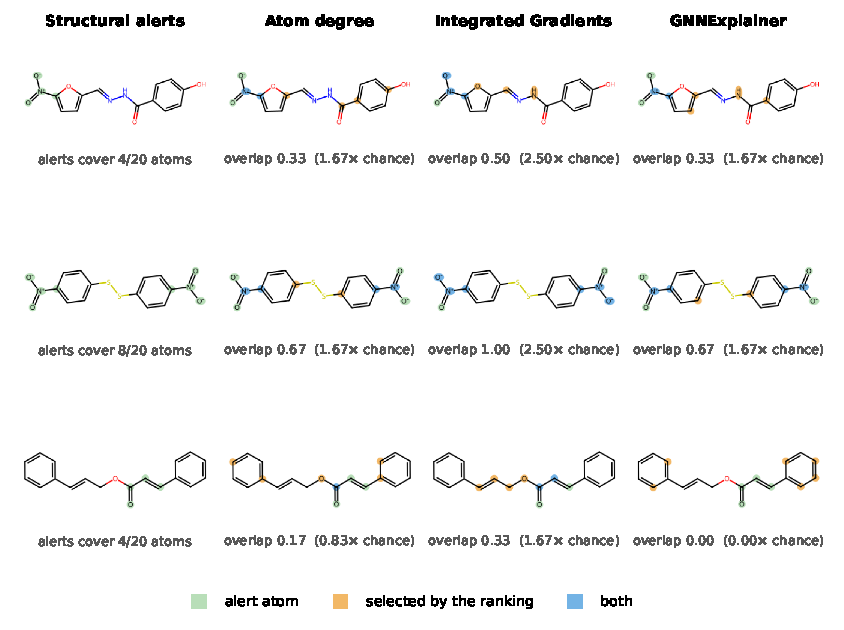
\includegraphics[width=0.96\textwidth]{figures/fig06_examples.pdf}
\caption{Alerts and three rankings on individual molecules. Molecules were chosen on
structure alone: from those in which the alerts cover between a fifth and a half of the
atoms, the three whose atom count is closest to the median. Each panel reports the overlap
and the chance level for that molecule.}
\label{fig:examples}
\end{figure}

\subsection{Controls on both model families}

The three control distributions differ from the untrained networks at the level of
distributions rather than merely of means (permutation $p < 0.001$ in each case), though the
separation is not absolute: a random weighting of atom features exceeds an untrained network
in one pair out of four (Supporting Information). The effect therefore requires message
passing and is not produced by the atom features or by the bit-to-atom map alone.


Under permuted labels both families lose their agreement. Graph models absorbed the
randomised labels in all fourteen repeats, reaching a training ROC-AUC of $0.874$ while
generalising to nothing ($0.492$ against the true test labels), and their attributions fall
to $1.036 \pm 0.074$, below the untrained distribution. The gradient-boosted model absorbed
its randomised labels more thoroughly ($0.973$) and its TreeSHAP attributions collapse to
$0.995 \pm 0.054$.

The graph result cannot be read as a statement about the labels. Fitting the permuted labels
required regularisation and early stopping to be switched off and the budget escalated, and
the models the drop is measured against were trained under none of that. Fitting the real
labels under the same regime gives $1.089$ ($1.021$ to $1.157$), an interval that contains
the permuted value of $1.036$. The drop is therefore attributable to the training regime
rather than to the randomisation, and we withdraw the reading that ascribed it to the labels.

Two caveats attach even to that. The matched arm reaches a training ROC-AUC of $0.9996$
against $0.874$ for the permuted one, so the two fitted their targets to different degrees
and the regimes are not identical. And eight models is a small arm. What the control now
supports is narrow: agreement is not immune to how a model is fitted, which is weaker than
what we previously claimed from it.

\subsection{The attribution rule and the representation}

The comparison between TreeSHAP and Integrated Gradients differs on two axes at once, the
attribution rule and the molecular representation. Fingerprint bits are substructure counters
and the alerts are substructures, so the fingerprint arm is aligned with the target by
construction. Applying Integrated Gradients to a multilayer perceptron over the same
fingerprints, and distributing the attributions through the same bit-to-atom map, separates
the two.

That model reaches $0.767$ test ROC-AUC and its attributions give $1.417 \pm 0.011$ under a
signed aggregation and $1.169 \pm 0.047$ under an absolute one. TreeSHAP on the fingerprint
model gives $1.542$ signed and $1.442$ absolute; the graph model gives $1.226$ absolute and
$1.068$ signed. These are single-model figures, computed on the designated model of the attribution
analysis so that the four conventions are comparable; the mean over the twenty models under
the absolute convention is $1.265$. Neither axis dominates, and the aggregation convention interacts with the
representation: under an absolute convention the graph model exceeds the fingerprint network,
and under a signed convention the order reverses by a wide margin. The difficulty is shared
between the gradient rule and the graph representation rather than belonging to either.

\subsection{Mask-based explanation}

GNNExplainer was measured on five trained models under three settings. Agreement is
$0.970 \pm 0.100$ at the default setting, $1.060 \pm 0.091$ with a longer optimisation and
$0.911 \pm 0.051$ with weaker mask regularisation, with nine of the fifteen runs below chance.
Pooled over the fifteen runs the method is therefore indistinguishable from chance and far
below the degree baseline,
rather than reliably below chance as a single model had suggested.

The mask entropy explains why. Normalised to the number of atoms it lies between $0.979$ and
$0.995$ under every setting, so the learned mask stays close to uniform and the ranking it
induces is arbitrary rather than uninformative. Repeating the method five times on one fixed
model gives a mean top-30\% Jaccard of $0.63$ against $0.99$ for Integrated Gradients, which
is deterministic given the model; the two are not comparable as measures of stability, and
the difference reflects the optimisation rather than the quality of the explanation.

\section{Predictive performance in full}

Under scaffold-disjoint cross-validation each of the 7,255 compounds receives one prediction
from a model that never saw its scaffold. GAT leads at $0.854$ ROC-AUC, GIN and XGBoost on
descriptors follow at $0.845$, and the random forest trails at $0.821$
(Figure~\ref{fig:accuracy}a, Table~\ref{tab:accuracy}). Eleven of the fifteen pairwise comparisons among the six main
models are resolved after correction for multiple testing.


\begin{figure}[htbp]
\centering
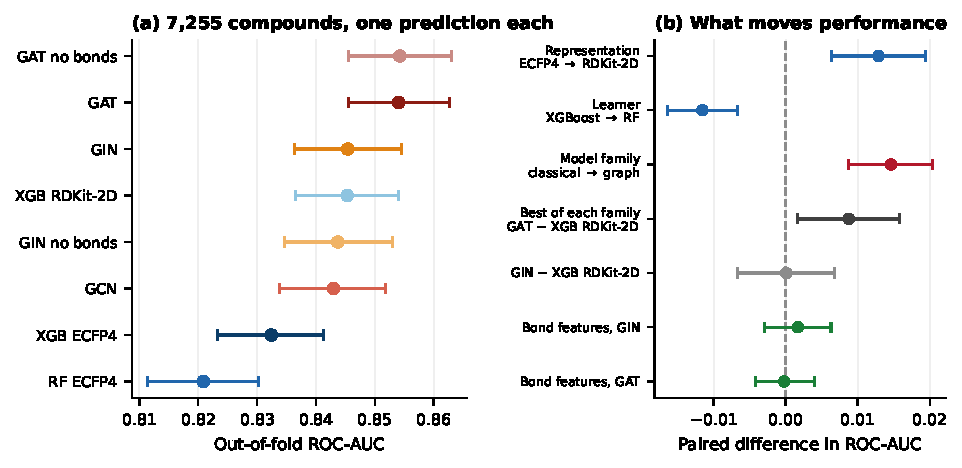
\includegraphics[width=0.98\textwidth]{figures/fig07_accuracy.pdf}
\caption{(a) Out-of-fold ROC-AUC with bootstrap intervals over all 7,255 compounds. (b)
Paired contrasts isolating the representation, the learner, the model family and bond
features.}
\label{fig:accuracy}
\end{figure}

\begin{table}[htbp]
\centering
\caption{Out-of-fold performance over all 7,255 compounds under scaffold-disjoint cross-validation. Every compound is predicted once by a model that never saw its scaffold.}
\label{tab:accuracy}
\footnotesize
\setlength{\tabcolsep}{4pt}
\begin{tabular}{lcccccc}
\toprule
Model & ROC-AUC & 95\% CI & PR-AUC & Sens. & Spec. & MCC \\
\midrule
GAT, no bond features & 0.854 & 0.845--0.863 & 0.863 & 0.800 & 0.755 & 0.555 \\
GAT & 0.854 & 0.846--0.863 & 0.866 & 0.833 & 0.724 & 0.562 \\
GIN & 0.845 & 0.836--0.854 & 0.853 & 0.779 & 0.786 & 0.564 \\
XGBoost (RDKit-2D) & 0.845 & 0.837--0.854 & 0.864 & 0.722 & 0.821 & 0.541 \\
GIN, no bond features & 0.844 & 0.835--0.853 & 0.843 & 0.819 & 0.729 & 0.552 \\
GCN & 0.843 & 0.834--0.852 & 0.842 & 0.779 & 0.765 & 0.543 \\
XGBoost (ECFP4) & 0.832 & 0.823--0.841 & 0.857 & 0.723 & 0.788 & 0.508 \\
Random forest (ECFP4) & 0.821 & 0.811--0.830 & 0.847 & 0.717 & 0.804 & 0.520 \\
\bottomrule
\end{tabular}
\begin{flushleft}\footnotesize Confidence intervals from 10,000 bootstrap resamples of the compounds, drawn jointly across models. 11 of 15 pairwise comparisons among the six main models are resolved after Holm correction.\end{flushleft}
\end{table}


What matters here is not the ordering but what moves it (Figure~\ref{fig:accuracy}b, Table~\ref{tab:contrasts}). Changing
the molecular representation of a fixed learner, from fingerprints to descriptors, is worth
$+0.013$ ROC-AUC (95\% CI $0.006$ to $0.019$, $p = 0.0002$). The gap between the two families
is $+0.0146$ ($0.0088$ to $0.0204$, $p < 0.001$) in favour of the graph models. The leading
member of each family, GAT and XGBoost on descriptors, differ by $+0.0088$ ($0.0016$ to
$0.0158$), a margin whose interval excludes zero but which does not survive Holm correction
across the fifteen pairwise comparisons ($p = 0.056$, Supporting Information). GIN, which carries the
attribution analysis below, is not the best graph model: it trails GAT by $0.0087$, and that
difference is resolved after correction ($p = 0.008$). Against XGBoost on descriptors GIN
differs by $+0.0001$ ($-0.007$ to $0.007$).

The picture is one of a narrow advantage rather than none, at the edge of what this design can
resolve.

\begin{table}[htbp]
\centering
\caption{Paired contrasts on the out-of-fold predictions, isolating the molecular representation, the learner, the model family and bond features.}
\label{tab:contrasts}
\small
\setlength{\tabcolsep}{4pt}
\begin{tabular}{lccc}
\toprule
Contrast & $\Delta$ ROC-AUC & 95\% CI & $p$ \\
\midrule
Representation: ECFP4 to RDKit-2D & +0.0129 & +0.0064 to +0.0195 & $<0.001$ \\
Learner: XGBoost to random forest & -0.0116 & -0.0164 to -0.0067 & $<0.001$ \\
Family: classical to graph & +0.0146 & +0.0088 to +0.0204 & $<0.001$ \\
Best of each family: GAT vs XGBoost (RDKit-2D) & +0.0088 & +0.0016 to +0.0158 & 0.014 \\
GIN vs XGBoost (RDKit-2D) & +0.0001 & -0.0067 to +0.0068 & 0.988 \\
GIN with and without bond features & +0.0017 & -0.0029 to +0.0063 & 0.471 \\
GAT with and without bond features & -0.0002 & -0.0043 to +0.0039 & 0.926 \\
\bottomrule
\end{tabular}
\begin{flushleft}\footnotesize $p$-values are uncorrected. Holm-corrected values for all fifteen pairwise comparisons among the six main models are given in the Supporting Information; under that correction the difference between the best model of each family gives $p = 0.056$.\end{flushleft}
\end{table}


One representational choice inside the graph family is inert: removing bond features changes
ROC-AUC by $+0.002$ for GIN ($p = 0.47$) and $-0.0002$ for GAT ($p = 0.93$). Whatever
separates the graph models from the fingerprint baseline, access to bond information is not
it.

Two further reference points frame the scale. A tuned logistic regression on the same
fingerprints reaches $0.761$ on the designated partition against $0.806$ for XGBoost on
descriptors, so feature interactions contribute less on this endpoint than is usually
assumed. The structural-alert classifier, which does no learning at all, reaches $0.678$;
57.7\% of test compounds carry at least one alert.

\section{Agreement across architectures and against performance}

Figure~\ref{fig:si_arch} gives the comparison against the model-free baseline for twenty
models in each of the three architectures. It is the same comparison the manuscript reports
numerically in Table~1, shown here so that the spread within each architecture is visible
beside the paired interval.

\begin{figure}[htbp]
\centering
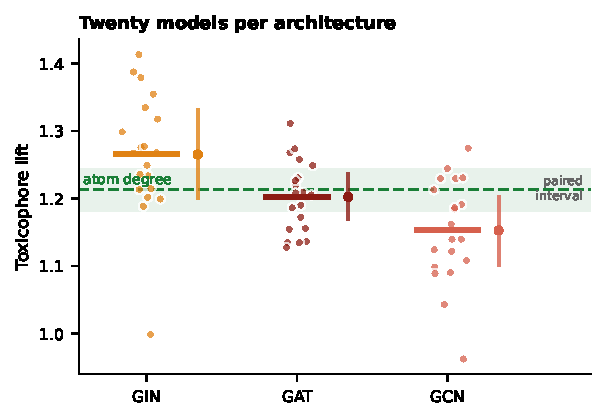
\includegraphics[width=0.62\textwidth]{figures/fig10_architectures.pdf}
\caption{Toxicophore agreement of twenty models in each of three architectures. The shaded
band is the baseline's bootstrap interval; the bar to the right of each group is the paired
interval on the difference from the baseline, drawn about it.}
\label{fig:si_arch}
\end{figure}

Figure~\ref{fig:si_models} shows the twenty GIN models against the baseline and the same
agreement against test performance. The second panel carries no claim: every
within-architecture interval contains zero, and the manuscript draws no conclusion from it.

\begin{figure}[htbp]
\centering
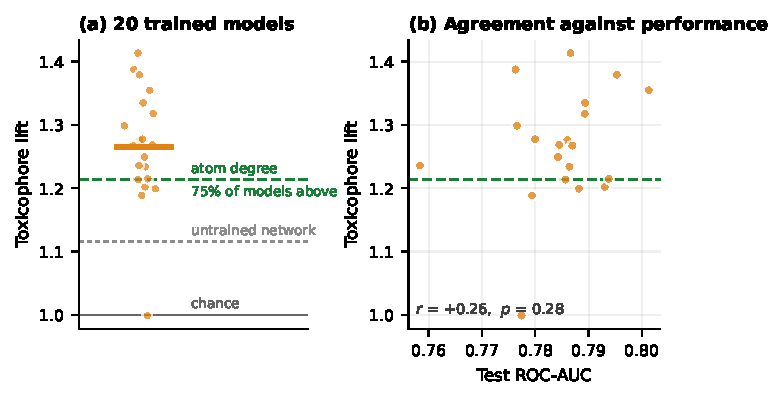
\includegraphics[width=0.86\textwidth]{figures/fig04_models.pdf}
\caption{(a) Toxicophore agreement of twenty independently trained models against the
model-free baseline. (b) The same agreement against test performance.}
\label{fig:si_models}
\end{figure}

\section{Supporting tables from the main analyses}

Table~\ref{tab:kfraction} gives the comparison against the degree ranking across five
retained fractions, which the manuscript summarises.

\begin{table}[htbp]
\centering
\caption{Agreement across retained fractions. Entries are the difference between a trained architecture and the degree ranking.}
\label{tab:kfraction}
\small
\setlength{\tabcolsep}{4pt}
\begin{tabular}{lcccc}
\toprule
Retained fraction & Degree lift & GIN & GAT & GCN \\
\midrule
0.10 & 1.202 & +0.229$^{*}$ & +0.136$^{*}$ & +0.055 \\
0.20 & 1.218 & +0.128$^{*}$ & +0.034 & -0.031 \\
0.30 & 1.214 & +0.052 & -0.011 & -0.061$^{*}$ \\
0.40 & 1.168 & +0.032 & -0.014 & -0.046$^{*}$ \\
0.50 & 1.108 & +0.040 & +0.000 & -0.014 \\
\bottomrule
\end{tabular}
\begin{flushleft}\footnotesize An asterisk marks a difference resolved at 0.05. The three cells at the smallest fraction carry a claim of presence and are corrected across that subfamily; the twelve at larger fractions carry a claim of absence, which a correction can only make harder to overturn, and are reported uncorrected. The $p$-values come from a recomputation with two hundred tie-breaks on every arm, which reproduces the differences shown here to within $0.001$ at the reference fraction.\end{flushleft}
\end{table}


Table~\ref{tab:replication} gives the aggregate difference from the degree ranking on each of
the three partitions drawn with the corrected splitter.

\begin{table}[htbp]
\centering
\caption{The threshold-free comparison repeated on three partitions drawn with the corrected splitter, five models each, against the designated partition of the manuscript.}
\label{tab:replication}
\footnotesize
\setlength{\tabcolsep}{4pt}
\begin{tabular}{lccccccc}
\toprule
Partition & $n$ & Random & Degree & GIN & $\Delta$ & 95\% CI & Tie \\
\midrule
Designated (size-ordered) & 237 & 0.492 & 0.580 & 0.637 & +0.056$^{*}$ & +0.019 to +0.093 & 0.868 \\
201 (random order) & 302 & 0.497 & 0.607 & 0.640 & +0.033 & -0.002 to +0.065 & 0.849 \\
202 (random order) & 349 & 0.499 & 0.571 & 0.646 & +0.075$^{*}$ & +0.018 to +0.124 & 0.895 \\
203 (random order) & 257 & 0.496 & 0.536 & 0.672 & +0.136$^{*}$ & +0.088 to +0.191 & 0.905 \\
\bottomrule
\end{tabular}
\begin{flushleft}\footnotesize An asterisk marks an interval excluding zero. Test sets of the three partitions share a mean Jaccard of 0.063 against 0.634 for the splitter used for the designated partition. The designated row carries twenty models; at five, resampling the twenty gives a mean interval width of 0.094 against 0.073, so the wider intervals here follow from the number of models rather than from the partition.\end{flushleft}
\end{table}


Table~\ref{tab:dod_replication} repeats the specificity check on those three partitions. It is
the analysis on which the manuscript withdraws the claim.

\begin{table}[htbp]
\centering
\caption{The specificity check repeated on the corrected partitions. Columns three and four are GIN's advantage over the degree ranking on each set.}
\label{tab:dod_replication}
\footnotesize
\setlength{\tabcolsep}{4pt}
\begin{tabular}{lccccc}
\toprule
Partition & Models & Mutagenic & Non-mutagenic & Difference & 95\% CI \\
\midrule
Designated & 10 & +0.089 & +0.039 & -0.050$^{*}$ & -0.091 to -0.011 \\
201 (corrected) & 5 & +0.056 & -0.033 & -0.089$^{*}$ & -0.152 to -0.031 \\
202 (corrected) & 5 & +0.116 & +0.127 & +0.011 & -0.056 to +0.070 \\
203 (corrected) & 5 & +0.067 & +0.053 & -0.014 & -0.067 to +0.039 \\
\bottomrule
\end{tabular}
\begin{flushleft}\footnotesize Five models on each corrected partition against ten on the designated one, so the intervals are wider. The pre-registered direction is negative. It holds on one of the three corrected partitions, is not resolved on a second, and reverses on the third.\end{flushleft}
\end{table}



Eleven tables referred to in the main text are collected here.

Table~\ref{tab:auroc} gives agreement as the area under the ROC curve for alert membership,
computed per model against the degree ranking on the ranking AUROC, which the main text
reports as primary.

\begin{table}[htbp]
\centering
\caption{Agreement as the area under the ROC curve for alert membership, computed per molecule and averaged, with the share of the top-30\% set that a tie at the cut decides.}
\label{tab:auroc}
\small
\setlength{\tabcolsep}{4pt}
\begin{tabular}{lccc}
\toprule
Ranking & $n$ & AUROC & Tie fraction \\
\midrule
atom degree & 1 & 0.580 & 0.87 \\
random ranking & 20 & 0.492 & 0.18 \\
trained GIN, IG & 20 & 0.637 & 0.19 \\
trained GAT, IG & 20 & 0.595 & 0.19 \\
trained GCN, IG & 20 & 0.598 & 0.20 \\
Gradient x Input & 20 & 0.610 & -- \\
Saliency & 20 & 0.644 & -- \\
\bottomrule
\end{tabular}
\begin{flushleft}\footnotesize A value of 0.5 is chance. The tie fraction is $0.87$ for atom degree, which takes five values across the dataset and fewer within a molecule. The floor is not zero: a continuous ranking still has the atom at the cut itself, which is $1/k$ and gives $0.18$ for a random ranking, so the attributions at about $0.19$ are effectively tie-free. Differences from the degree ranking, with their intervals and corrected $p$-values, are in Table~2 of the manuscript. TreeSHAP is absent because its atom-level scores were not retained.\end{flushleft}
\end{table}


Table~\ref{tab:regime_trained} places the trained models beside the model-free baseline under
the two reduced regimes of the alert library, which is the decomposition of the main text.

\begin{table}[htbp]
\centering
\caption{Trained models and the model-free baseline under the two reduced regimes of the alert library. Differences carry a paired resampling of molecules and models, as in Table~1 of the manuscript, which gives the same comparison over the full library; percentages are of the attainable above-chance range for that regime.}
\label{tab:regime_trained}
\footnotesize
\setlength{\tabcolsep}{4pt}
\begin{tabular}{llcccc}
\toprule
Regime & Arm & Lift & \% of range & $\Delta$ vs.\ degree & 95\% CI \\
\midrule
No fused aromatic ($n$ = 174) & Atom degree & 1.295 & 16 & -- & -- \\
 & Trained GIN & 1.737 & 40 & +0.442$^{*}$ & +0.304 to +0.588 \\
 & Trained GAT & 1.354 & 19 & +0.058 & -0.036 to +0.155 \\
 & Trained GCN & 1.184 & 10 & -0.112 & -0.236 to +0.020 \\
Fused aromatic only ($n$ = 97) & Atom degree & 1.172 & 31 & -- & -- \\
 & Trained GIN & 0.941 & -11 & -0.231$^{*}$ & -0.325 to -0.144 \\
 & Trained GAT & 1.109 & 19 & -0.062 & -0.135 to +0.006 \\
 & Trained GCN & 1.144 & 26 & -0.027 & -0.107 to +0.051 \\
\bottomrule
\end{tabular}
\begin{flushleft}\footnotesize An asterisk marks a difference resolved after Holm correction across the six tests in the two reduced regimes. Seven molecules the reduced libraries admit carry no stored attribution scores and are set aside, so every arm of a regime is scored on the same molecules; the counts given here are after that exclusion. GIN exceeds the baseline on the heteroatom-centred alerts and falls below it on the all-carbon pattern; the two effects have opposite signs and the full library averages them.\end{flushleft}
\end{table}


Table~\ref{tab:dod} reports the difference between the two evaluation sets under a signed
aggregation, the specificity check on the designated partition.

\begin{table}[htbp]
\centering
\caption{The difference between the two evaluation sets under a signed aggregation, with Holm correction across the three architectures.}
\label{tab:dod}
\footnotesize
\setlength{\tabcolsep}{4pt}
\begin{tabular}{lccccc}
\toprule
Architecture & Mutagenic & Non-mutagenic & Difference & 95\% CI & $p$ (Holm) \\
\midrule
GIN & +0.089 & +0.039 & -0.050$^{*}$ & -0.090 to -0.011 & 0.0366 \\
GAT & -0.032 & -0.055 & -0.024 & -0.065 to +0.018 & 0.5267 \\
GCN & +0.031 & +0.031 & +0.000 & -0.042 to +0.041 & 0.9747 \\
\bottomrule
\end{tabular}
\begin{flushleft}\footnotesize Columns two and three are each architecture's advantage over the degree ranking on that set. The pre-registered direction is negative: a model using the chemistry should rank alert atoms lower where they do not carry the endpoint. Ten models per architecture, 237 mutagenic and 168 non-mutagenic molecules.\end{flushleft}
\end{table}


Table~\ref{tab:shares} gives the share of each architecture's above-chance signal that the
model-free ranking accounts for.

\begin{table}[htbp]
\centering
\caption{The share of each architecture's above-chance signal that the model-free ranking supplies, with molecules and models resampled together.}
\label{tab:shares}
\small
\setlength{\tabcolsep}{4pt}
\begin{tabular}{lcc}
\toprule
Architecture & Share & 95\% CI \\
\midrule
GIN & 81\% & 64--107\% \\
GAT & 106\% & 89--127\% \\
GCN & 140\% & 104--208\% \\
\bottomrule
\end{tabular}
\begin{flushleft}\footnotesize The denominator is the architecture's own above-chance signal and is small for GCN, so the ratio is unstable there and the interval should be read as indicative. A share above 100\% would mean the baseline accounts for the whole of it; only for GCN does the interval lie entirely above that.\end{flushleft}
\end{table}


Table~\ref{tab:architectures} reports attribution across the three architectures with twenty
models each, together with the within-molecule association with degree.

\begin{table}[htbp]
\centering
\caption{Attribution across three architectures, twenty models each. $\rho$ is the within-molecule association between Integrated Gradients and atom degree; $r$ is the correlation between the per-molecule agreement of the architecture and of the degree ranking.}
\label{tab:architectures}
\small
\setlength{\tabcolsep}{4pt}
\begin{tabular}{lccc}
\toprule
Architecture & Lift & $\rho$(IG, degree) & $r$ per molecule \\
\midrule
GIN & 1.265 $\pm$ 0.092 & 0.429 & 0.824 \\
GAT & 1.203 $\pm$ 0.053 & 0.569 & 0.955 \\
GCN & 1.153 $\pm$ 0.077 & 0.496 & 0.889 \\
\bottomrule
\end{tabular}
\begin{flushleft}\footnotesize The comparison of each architecture against the baseline is given in Table~1 of the manuscript, where the uncertainty of the baseline is carried. The association with degree is weakest in GIN and strongest in GAT.\end{flushleft}
\end{table}


Table~\ref{tab:controls} collects the references and negative controls on the 237 evaluation
molecules at the reference retained fraction.

\begin{table}[htbp]
\centering
\caption{References and negative controls on the 237 evaluation molecules at a retained fraction of 30\%, in descending order of agreement.}
\label{tab:controls}
\small
\setlength{\tabcolsep}{4pt}
\begin{tabular}{lcccc}
\toprule
Reference & $n$ & Lift & Interval & \% of range \\
\midrule
Perfect ranking (ceiling) & -- & 1.914 & -- & 100.000 \\
TreeSHAP, fingerprint model & 1 & 1.542 & [1.462, 1.633] & 59.290 \\
Trained GIN, Integrated Gradients & 20 & 1.265 & $\pm$ 0.092 & 29.034 \\
Atom degree (model-free) & -- & 1.214 & $\pm$ 0.013 over tie-breaks & 23.352 \\
Untrained GIN & 500 & 1.116 & [0.989, 1.226] & 12.642 \\
Untrained GAT & 500 & 1.086 & [0.798, 1.240] & 9.394 \\
Untrained GCN & 500 & 1.037 & [0.758, 1.245] & 4.046 \\
GIN, permuted labels & 14 & 1.036 & $\pm$ 0.074 & 3.923 \\
Random values through the bit-to-atom map & 500 & 1.005 & [0.828, 1.186] & 0.570 \\
Random atom order & 500 & 1.000 & [0.956, 1.042] & -- \\
XGBoost, permuted labels & 16 & 0.995 & $\pm$ 0.054 & -- \\
GNNExplainer, three settings & 15 & 0.980 & $\pm$ 0.100 pooled & -- \\
Random weighting of atom features & 500 & 0.972 & [0.754, 1.217] & -- \\
\bottomrule
\end{tabular}
\begin{flushleft}\footnotesize Percentages are of the attainable above-chance range, from a lift of one to the ceiling of 1.914, measured from a ranking that places every alert atom first; rows at or below chance are left blank. The fingerprint arm is aligned with the alerts by construction, since its bits are substructure counters and the alerts are substructures. Against the untrained distribution, training raises the lift by +0.126 (95\% CI +0.057 to +0.202, Wilcoxon $p$ = 0.0013); 126 of 237 molecules improve. Superiority probabilities against a draw from the untrained GIN distribution: random atom order 0.96, random feature weighting 0.75, random through the bit map 0.84.\end{flushleft}
\end{table}


Table~\ref{tab:encoding} reports what removing atom degree from the input encoding does to the
association and to test performance.

\begin{table}[htbp]
\centering
\caption{Removing atom degree from the input encoding. $\rho$ is the within-molecule association between Integrated Gradients and atom degree, over 500 untrained initialisations and over twenty trained models; lift and test performance are for the trained models.}
\label{tab:encoding}
\small
\setlength{\tabcolsep}{4pt}
\begin{tabular}{lcccc}
\toprule
Encoding & Untrained $\rho$ ($n$=500) & Trained $\rho$ ($n$=20) & Lift & Test ROC-AUC \\
\midrule
Full (24 features) & 0.682 [0.440, 0.825] & 0.429 $\pm$ 0.109 & 1.265 $\pm$ 0.092 & 0.7849 \\
Degree removed (23) & 0.497 [0.138, 0.696] & 0.250 $\pm$ 0.129 & 1.174 $\pm$ 0.090 & 0.7861 \\
Degree and hydrogen count removed (22) & 0.656 [0.507, 0.772] & 0.421 $\pm$ 0.103 & 1.278 $\pm$ 0.083 & 0.7838 \\
\bottomrule
\end{tabular}
\begin{flushleft}\footnotesize Degree and hydrogen count are complementary at fixed valence, so removing degree alone leaves hydrogen count as an inverse proxy for it. Removing both restores the association, which is why the third row rather than the second is the clean comparison. Test performance is unchanged throughout.\end{flushleft}
\end{table}


Table~\ref{tab:correlation} decomposes what the per-molecule correlation with the degree
ranking measures.

\begin{table}[htbp]
\centering
\caption{What the per-molecule correlation with the degree ranking measures. The first column is the raw correlation of per-molecule overlaps, the second removes each molecule's chance coverage, and the third is the agreement between the atoms actually selected.}
\label{tab:correlation}
\small
\setlength{\tabcolsep}{4pt}
\begin{tabular}{lccc}
\toprule
Compared with degree & $r$ & $r$ given chance coverage & Jaccard of selected atoms \\
\midrule
untrained GIN & 0.943 & 0.567 & -- \\
trained GIN & 0.826 & 0.309 & 0.331 \\
random ranking & 0.807 & -0.033 & 0.189 \\
\bottomrule
\end{tabular}
\begin{flushleft}\footnotesize A random ranking correlates with the degree ranking at 0.81 on the raw measure, so most of that quantity reflects the shared bound rather than agreement. The partial correlation and the Jaccard are the informative columns.\end{flushleft}
\end{table}


Table~\ref{tab:performance} sets agreement with the alerts against predictive performance
within each architecture.

\begin{table}[htbp]
\centering
\caption{Agreement with the alerts against predictive performance, within each architecture and pooled.}
\label{tab:performance}
\small
\setlength{\tabcolsep}{4pt}
\begin{tabular}{lcccc}
\toprule
Scope & $n$ & ROC-AUC range & $r$ & 95\% CI \\
\midrule
GIN & 20 & 0.758--0.801 & 0.256 & -0.21 to +0.63 \\
GAT & 20 & 0.759--0.803 & 0.272 & -0.19 to +0.64 \\
GCN & 20 & 0.751--0.793 & 0.293 & -0.17 to +0.65 \\
All three & 60 & 0.751--0.803 & 0.394 & +0.16 to +0.59 \\
\bottomrule
\end{tabular}
\begin{flushleft}\footnotesize Within an architecture no relation is resolvable. The pooled correlation is confounded with architecture identity, since GIN has both the highest mean performance and the highest agreement and GCN the lowest of each.\end{flushleft}
\end{table}


Table~\ref{tab:intervals} gives the model-free baseline with its interval, and the association
with degree on the second molecule set.

\begin{table}[htbp]
\centering
\caption{The model-free baseline with its interval, and the association with degree on a second set of molecules that carries no alert annotation.}
\label{tab:intervals}
\small
\setlength{\tabcolsep}{4pt}
\begin{tabular}{lccc}
\toprule
Quantity & Estimate & 95\% CI & Molecules positive \\
\midrule
Degree ranking, lift (molecules resampled) & 1.214 & 1.183--1.243 & -- \\
$\rho$(IG, degree), untrained, Ames test (evaluation set) ($n$ = 200 draws) & 0.685 & -- & 98.5\% \\
$\rho$(IG, degree), untrained, BBBP ($n$ = 200 draws) & 0.646 & -- & 99.0\% \\
\bottomrule
\end{tabular}
\begin{flushleft}\footnotesize The shares of each architecture's above-chance signal are given with their intervals in Table~\ref{tab:shares}. The second set is drawn from a blood--brain barrier penetration dataset; the association with degree needs neither labels nor alerts.\end{flushleft}
\end{table}


Table~\ref{tab:specificity} reports the mutagenic and non-mutagenic evaluation sets under the
signed aggregation the specificity check requires.

\begin{table}[htbp]
\centering
\caption{Mutagenic and non-mutagenic evaluation sets under a signed aggregation, which is required because an absolute sum cannot distinguish an atom pushing the prediction towards mutagenic from one pushing the other way.}
\label{tab:specificity}
\footnotesize
\setlength{\tabcolsep}{4pt}
\begin{tabular}{llccccc}
\toprule
Set & Ranking & $n$ & Models & AUROC & $\Delta$ vs.\ degree & 95\% CI \\
\midrule
Mutagenic & atom degree & 237 & 1 & 0.580 & -- & -- \\
Mutagenic & trained GIN & 237 & 10 & 0.669 & +0.089$^{*}$ & +0.049 to +0.126 \\
Mutagenic & trained GAT & 237 & 10 & 0.549 & -0.032 & -0.071 to +0.006 \\
Mutagenic & trained GCN & 237 & 10 & 0.611 & +0.031$^{*}$ & +0.0002 to +0.0609 \\
Non-mutagenic & atom degree & 168 & 1 & 0.590 & -- & -- \\
Non-mutagenic & trained GIN & 168 & 10 & 0.629 & +0.039 & -0.006 to +0.083 \\
Non-mutagenic & trained GAT & 168 & 10 & 0.534 & -0.055$^{*}$ & -0.094 to -0.018 \\
Non-mutagenic & trained GCN & 168 & 10 & 0.621 & +0.031 & -0.005 to +0.066 \\
\bottomrule
\end{tabular}
\begin{flushleft}\footnotesize Ten models per architecture. A model using the chemistry should rank alert atoms lower where they do not carry the endpoint; the degree ranking, which cannot see the label, should behave alike in both sets, and does.\end{flushleft}
\end{table}


\section{The structural ranking panel on the corrected partitions}

Atom degree was chosen as the baseline on a screen of eleven structural rankings across three
regimes of the alert library, carried out on the designated partition. Because the screen and
every comparison that followed it used the same molecules, the selection could in principle be
a property of that partition. It is repeated here on the three partitions of the replication
analysis, drawn with the random-order splitter.

None of the eleven rankings needs a model, so the repetition costs nothing beyond the scoring.
Each ranking is computed from the molecular graph alone, atoms are retained at the same
fraction of $0.30$, ties at the cut are broken at random and averaged over two hundred draws,
and the interval on each lift comes from ten thousand resamples of the molecules. A ranking
passes a regime when the lower bound of that interval lies above chance for the regime. The
designated partition is included as a control: the rewritten scoring path reproduces the
published lifts to within $0.002$.

Table~\ref{tab:si_panel} repeats that screen on the three partitions drawn with the corrected
splitter.

\begin{table}[htbp]
\centering
\caption{The screen that selected the baseline, repeated on three partitions drawn with the corrected splitter. Columns two to four are the lift of the degree ranking in each regime.}
\label{tab:si_panel}
\small
\setlength{\tabcolsep}{4pt}
\begin{tabular}{lcccl}
\toprule
Partition & Full & Heteroatom & Fused only & Above chance in all three \\
\midrule
Designated & 1.213 & 1.276 & 1.161 & degree \\
201 (corrected) & 1.215 & 1.356 & 1.113 & degree \\
202 (corrected) & 1.246 & 1.342 & 1.108 & degree \\
203 (corrected) & 1.196 & 1.254 & 1.169 & degree \\
\bottomrule
\end{tabular}
\begin{flushleft}\footnotesize Eleven rankings were scored in each regime on each partition. Atom degree is the only one whose interval lies above chance under all three regimes, on every partition including the designated one, so the selection rule transports out of the partition on which it was applied. The designated row is a recomputation along the path of this analysis and agrees with the values in the main text to within 0.002.\end{flushleft}
\end{table}


\section{What the non-nested hyperparameter search cost}

The hyperparameter search was run once on the designated partition and the selected
configurations were reused in the cross-validation, so the 725 compounds of that partition's
validation set appear in the test folds. Whether this affects the comparison between models,
rather than only their absolute level, can be measured from the stored predictions.

Every compound has an out-of-fold prediction from every model. Splitting those predictions
into the 725 compounds the search evaluated against and the 6,530 it did not, and scoring each
model on both, gives a per-model optimism. Intervals come from ten thousand resamples of the
compounds within each subset, with the same draws used for every model so that a difference
between two of them can be read from the same resampling. The quantity of interest is the
difference between the family means, which carries its own interval from those shared draws.

Only the validation compounds are treated as exposed. The training compounds of the designated
partition were seen by the search as well, but the cross-validation refits every model from
scratch within each fold, so a compound in a fold's training set contributes to that fold's
model whether or not the search saw it; what the search could have overfitted is the
configuration, and the configuration was chosen against the validation set alone.

The two subsets are not matched on difficulty, so the absolute gap between them is not
interpretable. Only its spread across models bears on a contrast between models, and the
search set is a tenth of the data, so an optimism difference translates into about a tenth of
itself on the pooled estimate.

Table~\ref{tab:si_optimism} gives out-of-fold performance on the 725 compounds the search saw
and on the 6,530 it did not, per model.

\begin{table}[htbp]
\centering
\caption{Out-of-fold performance on the 725 compounds the hyperparameter search saw and on the 6,530 it did not.}
\label{tab:si_optimism}
\footnotesize
\setlength{\tabcolsep}{4pt}
\begin{tabular}{llccccc}
\toprule
Model & Family & All & Search set & Rest & Optimism & 95\% CI \\
\midrule
XGBoost & Classical & 0.832 & 0.851 & 0.831 & +0.020 & -0.010 to +0.048 \\
RandomForest & Classical & 0.821 & 0.861 & 0.818 & +0.044 & +0.015 to +0.071 \\
XGBoost\_RDKit2D & Classical & 0.845 & 0.862 & 0.844 & +0.018 & -0.010 to +0.045 \\
GCN & Graph & 0.843 & 0.844 & 0.843 & +0.001 & -0.030 to +0.030 \\
GIN & Graph & 0.845 & 0.859 & 0.844 & +0.015 & -0.015 to +0.043 \\
GAT & Graph & 0.854 & 0.842 & 0.855 & -0.013 & -0.044 to +0.016 \\
\bottomrule
\end{tabular}
\begin{flushleft}\footnotesize The two subsets are not matched on difficulty, so the absolute gap is not interpretable; only its spread across models is. The graph models carry -0.027 (-0.043 to -0.011) less optimism than the classical ones, so the family contrast of $+0.0146$ is if anything suppressed by the non-nested search rather than produced by it. The search set is a tenth of the data, so the effect on the pooled contrast is about a tenth of that difference; the figure here is not directly comparable with the contrast.\end{flushleft}
\end{table}


\section{The fused-aromatic alert}

The pattern supplying most of the alert atoms is our own encoding of a class that Kazius and
co-workers describe rather than specify. Table~\ref{tab:si_pattern} repeats the regime
analysis under three readings of it, obtained by merging aromatic rings that share atoms into
systems and thresholding on the number of rings in a system. This is not a named
substructure: a query for anthracene matches linear acenes only and would miss phenanthrene,
chrysene and benzo[a]pyrene, whose rings are fused angularly and which carry the mechanism
that matters here.

\begin{table}[htbp]
\centering
\caption{The regime split under three readings of the fused-aromatic alert, from ring perception rather than a named substructure.}
\label{tab:si_pattern}
\footnotesize
\setlength{\tabcolsep}{4pt}
\begin{tabular}{llcccccc}
\toprule
Reading & Molecules & Regime & $n$ & Degree & GIN & $\Delta$ & 95\% CI \\
\midrule
Two or more fused rings & 140 & Fused only & 127 & 1.189 & 0.892 & -0.297$^{*}$ & -0.391 to -0.203 \\
Two or more fused rings & 140 & Fused removed & 174 & 1.214 & 1.732 & +0.517$^{*}$ & +0.364 to +0.683 \\
Three or more & 89 & Fused only & 76 & 1.165 & 0.939 & -0.225$^{*}$ & -0.318 to -0.139 \\
Three or more & 89 & Fused removed & 174 & 1.264 & 1.729 & +0.465$^{*}$ & +0.320 to +0.621 \\
Four or more & 47 & Fused only & 34 & 1.108 & 0.917 & -0.192$^{*}$ & -0.277 to -0.115 \\
Four or more & 47 & Fused removed & 174 & 1.287 & 1.735 & +0.448$^{*}$ & +0.307 to +0.597 \\
\bottomrule
\end{tabular}
\begin{flushleft}\footnotesize The molecule set of the fused-removed column is the same under all three readings, but the alert atoms are not: each reading withdraws a different set of atoms from the library, so the degree ranking moves while the model does not. Aromatic rings sharing atoms are merged into systems and thresholded on the number of rings, so angular systems such as phenanthrene and benzo[a]pyrene are counted; a query for a named linear acene would miss them. The sign of the difference is the same under all three readings.\end{flushleft}
\end{table}


\section{The attribution baseline}

Integrated Gradients is computed in the main text from a zero baseline, which for one-hot
inputs lies outside the space the model was trained on. Table~\ref{tab:si_baseline} repeats
the untrained measurement from the dataset-average atom vector instead. Over five hundred draws with percentile intervals, the association with
degree is lower under the on-manifold baseline and survives under every encoding, but the
ordering of the two reduced encodings reverses: under the zero baseline removing degree
together with hydrogen count restores the association, and under the on-manifold baseline it
does not. The main text reports this and reads the ablation accordingly.

\begin{table}[htbp]
\centering
\caption{Sensitivity of the untrained association to the Integrated Gradients baseline, over five hundred initialisations with percentile intervals.}
\label{tab:si_baseline}
\small
\setlength{\tabcolsep}{4pt}
\begin{tabular}{lcc}
\toprule
Encoding & $\rho$, zero baseline & $\rho$, mean baseline \\
\midrule
Full (24 features) & 0.682 [0.440, 0.825] & 0.673 [0.529, 0.765] \\
Degree removed (23) & 0.497 [0.138, 0.696] & 0.603 [0.416, 0.726] \\
Degree and hydrogen count removed (22) & 0.656 [0.507, 0.772] & 0.576 [0.402, 0.708] \\
\bottomrule
\end{tabular}
\begin{flushleft}\footnotesize A zero baseline is off-manifold for one-hot inputs. The ordering of the two reduced encodings reverses between the baselines, which is why the encoding ablation is read as bounding rather than settling the question.\end{flushleft}
\end{table}


\section{The second molecule set}

The association between an untrained network's attributions and atom degree was repeated on
molecules from the blood--brain barrier penetration dataset distributed with MoleculeNet.
From the compounds that parse and carry at least four heavy atoms, 299 were drawn at random
under a fixed seed; no property or label was used in the selection, since the measurement
needs neither.

\section{Bit-to-atom ambiguity and the effect of training}

\begin{table}[htbp]
\centering
\caption{Ambiguity of the bit-to-atom map, and what predicts the change in agreement produced by training.}
\label{tab:si_misc}
\small
\setlength{\tabcolsep}{4pt}
\begin{tabular}{lr}
\toprule
Quantity & Value \\
\midrule
Fingerprint bits carrying more than one environment & 100.0\% \\
Mean environments per shared bit & 11.9 \\
Most environments on one bit & 33 \\
Regression on the change in agreement: alert coverage & $\beta$ = -0.417, $p$ $<$ 0.001 \\
Regression on the change in agreement: heteroatom fraction & $\beta$ = +0.795, $p$ $<$ 0.001 \\
Regression on the change in agreement: degree spread & $\beta$ = -0.667, $p$ $<$ 0.001 \\
Regression $R^2$ & 0.491 \\
\bottomrule
\end{tabular}
\begin{flushleft}\footnotesize The regression target is the difference between the trained and untrained overlap for the same molecule. All variance inflation factors are below 2.6.\end{flushleft}
\end{table}


Every one of the 2,048 fingerprint bits carries more than one atom environment somewhere in
the dataset. A TreeSHAP value assigned to a bit is therefore shared among chemically distinct
environments, and distributing it to atoms in one molecule imports information from others.
This works against the fingerprint arm, so its strong performance in the main text is a lower
bound rather than an upper one.

The regression takes as its target the difference between the trained and untrained overlap
for the same molecule, which is the quantity the claim concerns. It has $n = 237$ and three
predictors, all standardised, fitted by ordinary least squares with no selection: the
heteroatom fraction, the within-molecule standard deviation of atom degree, and the fraction
of atoms covered by alerts. Coefficients, standard errors and variance inflation factors are
given in Table~\ref{tab:si_misc}. An earlier specification
used the raw overlap while including alert coverage as a predictor; since chance overlap is
alert coverage, that specification was close to tautological and is not reported.

\section{Code and data}

The dataset is publicly available through the Therapeutics Data Commons. The pipeline is
released as notebooks covering data preparation and hyperparameter search, final
fitting, the multi-partition benchmark, cross-validation, attribution and negative controls,
structural baselines, the architecture and encoding comparisons, the threshold-free and
regime analyses, and the replication on corrected partitions. All random seeds
are fixed. Model weights, the raw atom-level attributions of the graph models and the fold
assignments are retained, a manifest records which stage produced each result file, and a
companion file lists every quantity quoted in the manuscript. The atom-level TreeSHAP values
were not kept.
The repository is named in the Data and Software Availability statement of the manuscript.

\bibliography{references}

\end{document}
